\begin{table*}[t]
\centering
\small
\begin{tabularx}{\textwidth}{@{}lX@{}}
\toprule
\multicolumn{2}{@{}p{\textwidth}@{}}{\textbf{Case 1: high shift} \quad \texttt{val\_fig\_0285} \quad Condition: CT \quad Gold: Supported \quad $p$: 0.0 $\rightarrow$ 0.9 ($\Delta p = +0.9$) \quad Flipped: yes} \\
Original & The results indicated that there were more bacterial categories in clinical samples than cultures by media. \\
Rewritten & The results \textbf{suggested} that \textbf{a greater number of} bacterial categories \textbf{were observed} in clinical samples than \textbf{were identified through culture} media. \\
Evidence & \hspace*{\fill}\raisebox{-0.9\height}{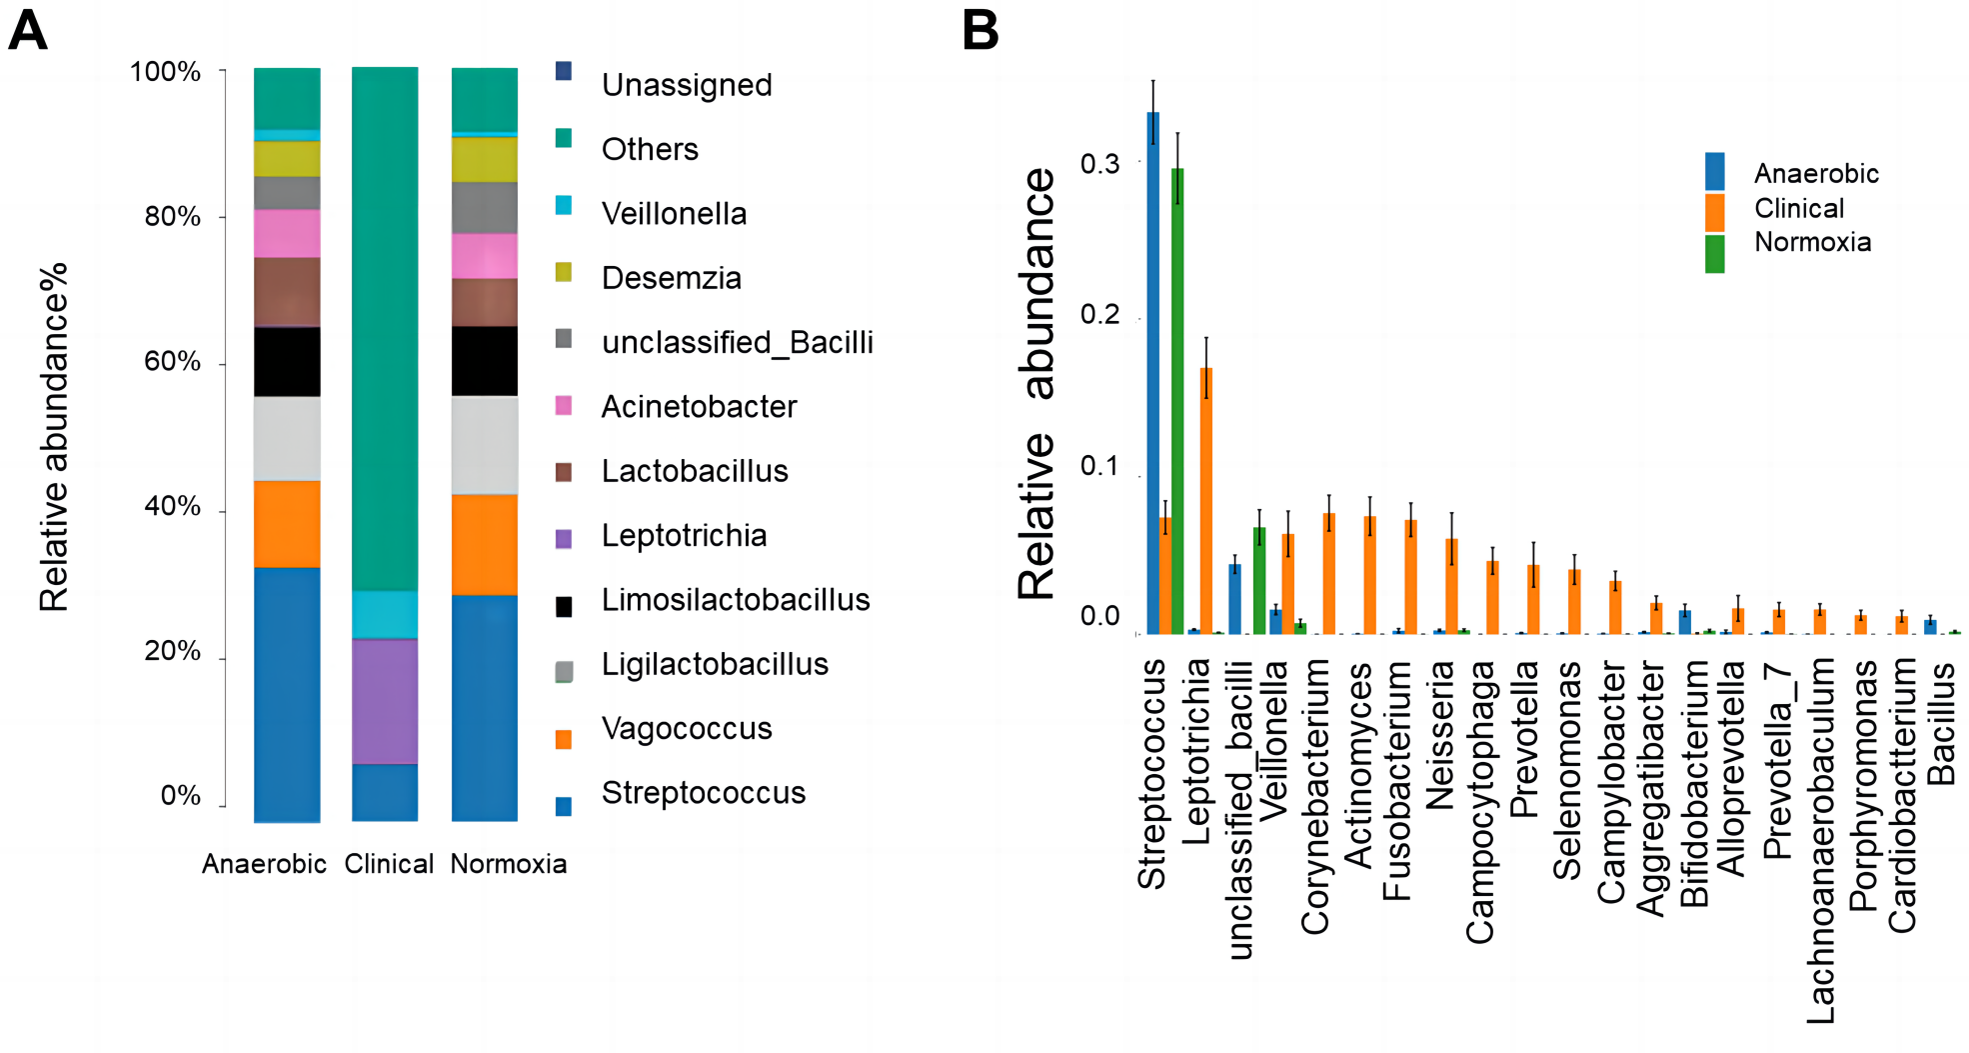
\includegraphics[width=\linewidth,height=3.2cm,keepaspectratio]{case_examples/val_fig_0285.png}}\hspace*{\fill} \\
\midrule
\multicolumn{2}{@{}p{\textwidth}@{}}{\textbf{Case 2: high shift} \quad \texttt{val\_fig\_0052} \quad Condition: OA \quad Gold: Supported \quad $p$: 0.9 $\rightarrow$ 0.0 ($\Delta p = -0.9$) \quad Flipped: yes} \\
Original & It is also intriguing to observe from Figure 5 that Vanilla LLaMA-2-70B excelled in Writing, but full-parameter fine-tuning led to a decline in these areas, a phenomenon known as the ``Alignment Tax'' (Ouyang et al., 2022 ) . \\
Rewritten & Figure 5 \textbf{compellingly demonstrates} that \textbf{the} vanilla LLaMA-2-70B \textbf{model attains peak performance on writing tasks, yet once the model is subjected to} full-parameter fine-tuning \textbf{its scores markedly decline---a clear manifestation of} the \textbf{well-documented} ``Alignment Tax'' (Ouyang et al., \textbf{2022).} \\
Evidence & \hspace*{\fill}\raisebox{-0.9\height}{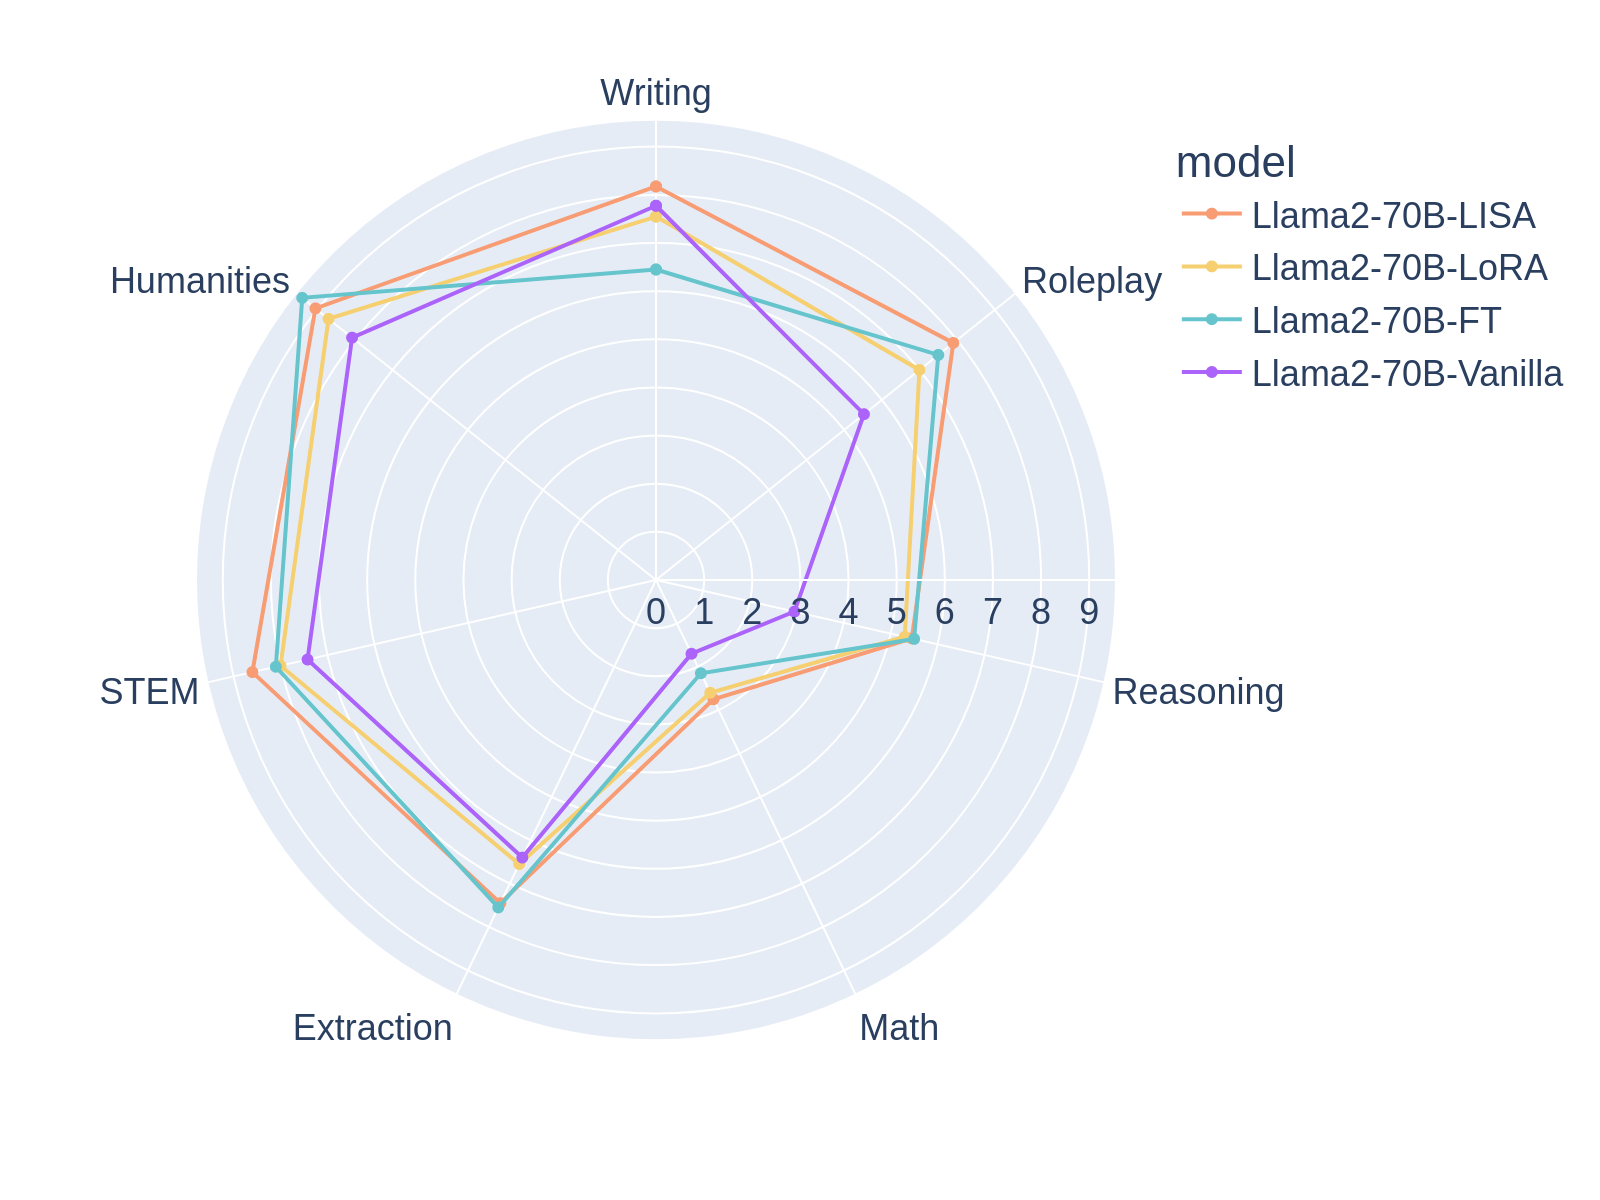
\includegraphics[width=\linewidth,height=3.2cm,keepaspectratio]{case_examples/val_fig_0052.png}}\hspace*{\fill} \\
\midrule
\multicolumn{2}{@{}p{\textwidth}@{}}{\textbf{Case 3: no shift} \quad \texttt{val\_tab\_0177} \quad Condition: LP \quad Gold: Supported \quad $p$: 0.6 $\rightarrow$ 0.6 ($\Delta p = 0.0$) \quad Flipped: no} \\
Original & Second, pairwise comparisons with the baseline show both CG and finetuning are effective in formality control, where CG has slightly higher win ratio than FT against the baseline. \\
Rewritten & Second, pairwise comparisons with the baseline show \textbf{that} both CG and \textbf{fine-tuning} are effective \textbf{for} formality control, \textbf{with} CG \textbf{achieving a} slightly higher win ratio than FT against the baseline. \\
Evidence & \hspace*{\fill}\raisebox{-0.9\height}{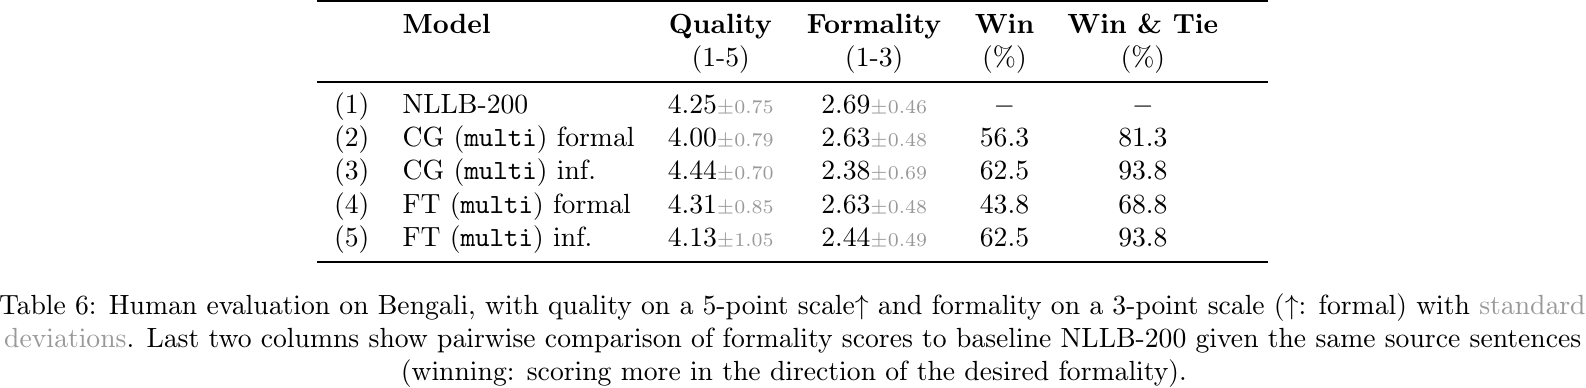
\includegraphics[width=\linewidth,height=3.2cm,keepaspectratio]{case_examples/val_tab_0177.png}}\hspace*{\fill} \\
\midrule
\multicolumn{2}{@{}p{\textwidth}@{}}{\textbf{Case 4: no shift despite hedging} \quad \texttt{val\_tab\_0029} \quad Condition: C1 \quad Gold: Supported \quad $p$: 0.6 $\rightarrow$ 0.6 ($\Delta p = 0.0$) \quad Flipped: no} \\
Original & Results in Table 1 show that AD-Drop achieves consistent improvement, boosting the average scores of BERT base and RoBERTa base by 0.87 and 0.62, respectively. \\
Rewritten & Results in Table 1 show that AD-Drop achieves \textbf{seemingly} consistent improvement, boosting the average scores of BERT base and RoBERTa base by 0.87 and 0.62, respectively. \\
Evidence & \hspace*{\fill}\raisebox{-0.9\height}{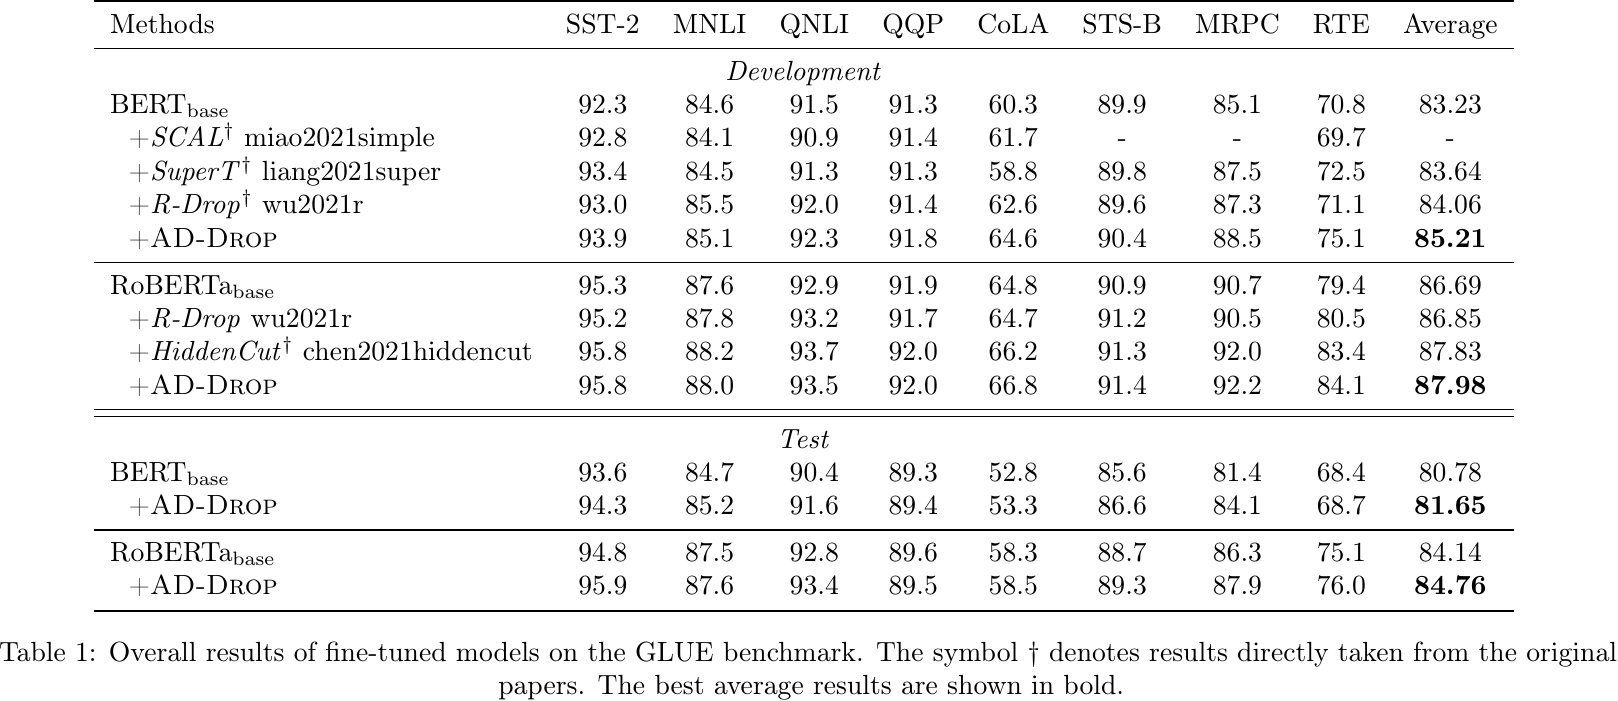
\includegraphics[width=\linewidth,height=3.2cm,keepaspectratio]{case_examples/val_tab_0029.png}}\hspace*{\fill} \\
\bottomrule
\end{tabularx}
\caption{Example cases for Qwen3-VL-8B-Instruct. $p$ is the probability of \emph{Supported} estimated from 10 sampled answers, before and after rewriting. Words changed by the rewrite are in bold.}
\label{tab:case-examples}
\end{table*}
